		% !TeX spellcheck = nl_NL-Dutch
\documentclass{kulakarticle}
\usepackage[dutch]{babel}
\usepackage{hyperref}
\usepackage{siunitx}
\usepackage{graphicx}
\title{Mijn eerste \LaTeX-document}
\author{Tim Wyckaert}
\date{\today}



\begin{document}
	
	Afstanden van het testgebied 
	\begin{figure}
		\centering
		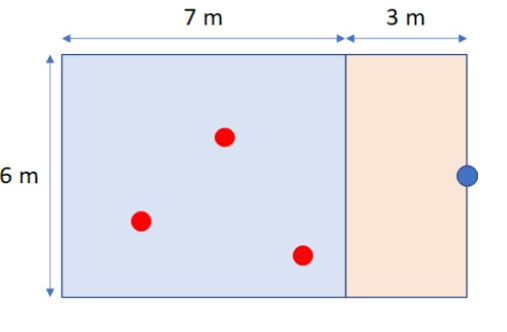
\includegraphics[width=.62\textwidth]{afstanden}
	\end{figure}

	ontwerp brandblusser met rand
	\begin{figure}
		\centering
		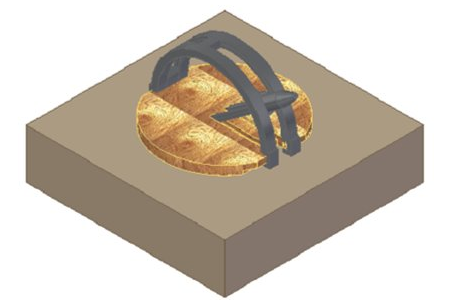
\includegraphics[width=.62\textwidth]{bompakanon}
	\end{figure}

	ontwerp brandblusser zonder rand
	\begin{figure}
		\centering
		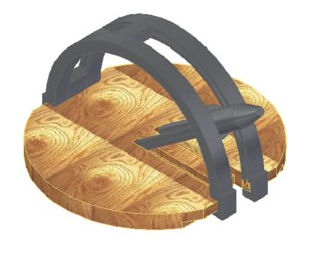
\includegraphics[width=.62\textwidth]{bompakanon_2}
	\end{figure}

	mondstuk
	\begin{figure}
	\centering
	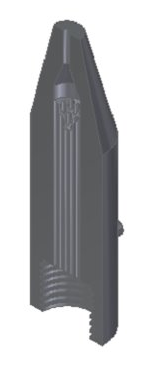
\includegraphics[width=.22\textwidth]{mondstuk}
	\end{figure}


	hoekprobleem voor plaatsbepaling van de camera
	\begin{figure}
		\centering
		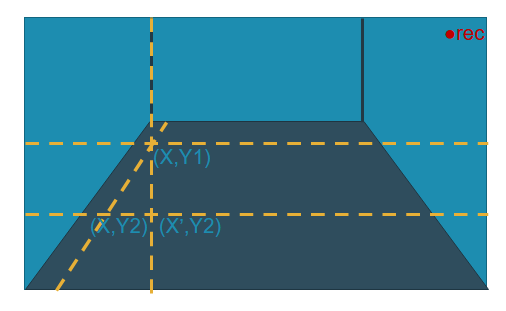
\includegraphics[width=.62\textwidth]{hoekprobleem}
	\end{figure}

	plaatsbepaling van de camera
	\begin{figure}
		\centering
		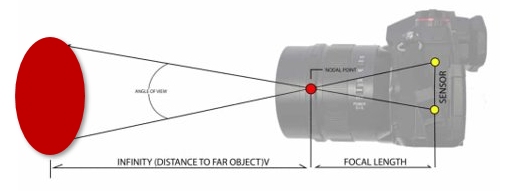
\includegraphics[width=.62\textwidth]{plaatsbepaling}
	\end{figure}

	Mogelijke kleurenspectrum van de camera
	\begin{figure}
		\centering
		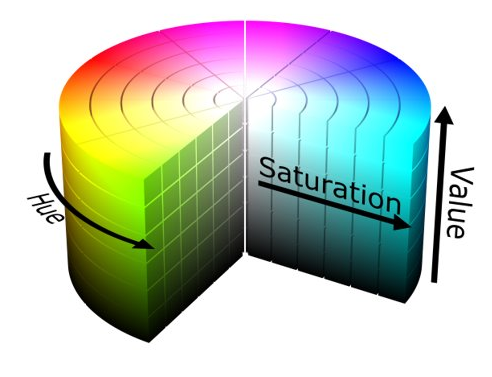
\includegraphics[width=.62\textwidth]{saturation}
	\end{figure}


	verschillende banen van de waterstraal afhankelijk van de beginsnelheid
	
	\begin{figure}
	\centering
	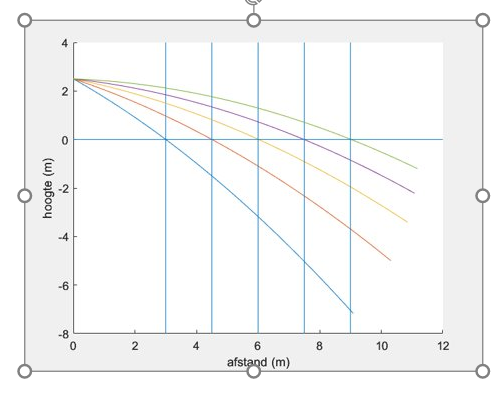
\includegraphics[width=.62\textwidth]{waterbaan}
	\end{figure}
	
	
	beweging van de straal met de werking van verschillende krachten
	\begin{figure}
	\centering
	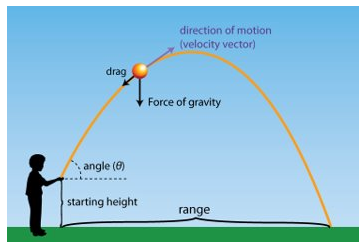
\includegraphics[width=.62\textwidth]{baanbeweging}
	\end{figure}





\end{document}